
\ccDefGlobalScope{CGAL::}

\section{Introduction}

A subset $S \subseteq \R^d$ is convex if for any two points $p$ and $q$ in the set the line segment with endpoints $p$ and $q$ is contained in $S$. The convex hull of a set $S$ is the smallest convex set containing $S$. The convex hull of a finite set of points $A \in \R^d$ is a convex polytope with vertices in $A$. A point in $A$ is an extreme point \ccIndexMainItemDef{extreme point} (with respect to $A$) iff it is a vertex of the convex hull of $A$. This also means that a point in $A$ is an extreme point iff it is not contained in the convex hull of all the other points in $A$.

This chapter describes the functions and class provided in \cgal\ for computing the extreme points of arbitrary dimensional point sets. There are two ways to compute extreme points of arbitrary dimensional point sets in \cgal: using a static algorithm or using the dynamic class \ccc{Extreme_points_d<Traits>}. The class \ccc{Extreme_points_d<Traits>} maintains a semi-dynamic point set and answers extreme point queries.

\section{Static extreme points computations}
The function \ccc{extreme_points_d_simple} computes the extreme points of a d-dimensional point set using a straightforward algorithm based on linear programming.

For point sets with low extreme point density Dul\'a and Helgason invented an output-sensitive algorithm \cite{cgal:dh-pifch-96}. The function \ccc{extreme_points_d_dula_helgason} provides an implementation of this algorithm.

\ccExample
The following program computes the extreme points of a set of 500 random points chosen from a 10-dimensional iso box uniformly at random. The same results could be achieved by substituting the function \ccc{CGAL::extreme_points_d_dula_helgason} by \ccc{CGAL::extreme_points_d_simple}. 

Note that although \ccc{double} is used here as the field number type for the Kernel doesn't mean that the algorithm will not be exact. Internally an appropriate exact number type is used for intermediate results. 

\ccIncludeExampleCode{Extreme_points_d/extreme_points_d_dula_helgason.cpp}


\section{Extreme points computations for a dynamically increasing point set}
For extreme point queries on a growing point set the class \ccc{Extreme_points_d<Traits>} can be used. This class maintains a set of points in an arbitrary (but fixed) dimension. Extreme point computations are done lazily (i.e. only on extreme point queries) and the result of the last extreme point computation is kept and used in the next computation.

The class can also classify query points in relation to the convex hull of the current point set. Such a query point is either one of the extreme points, some other point inside the convex hull or completely outside the convex hull (which means it would be an extreme point when added to the point set).

\ccExample
The following program demonstrates the usage of \ccc{Extreme_points_d<Traits>}. Randomly chosen points are added to the current point set in multiple batches. In between, the extreme points of the current set are calculated and some classify queries are made.

\ccIncludeExampleCode{Extreme_points_d/Extreme_points_d.cpp}


\section{Demo}

This package comes with an interactive demo of \ccc{Extreme_points_d<Traits>}. For simplicity and for better interaction and imagination the demo operates only with 2-dimensional points. Source code: \ccc{<CGAL_ROOT>/demo/Extreme_points_d/Extreme_points_2.cpp}).

\begin{figure}[htbp]
\begin{ccTexOnly}
\begin{center}
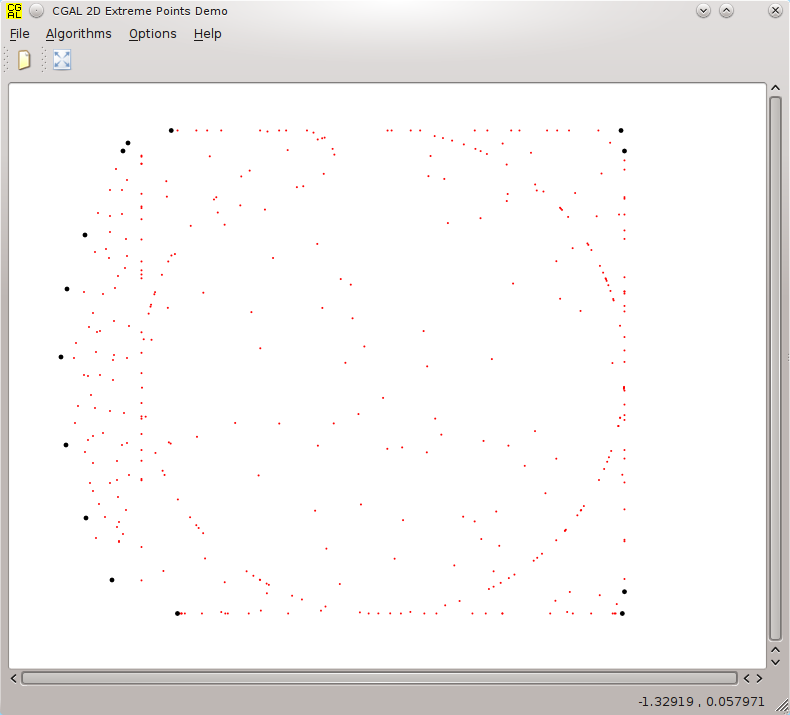
\includegraphics[width=\textwidth]{Extreme_points_d/extreme_points_demo.png}
\end{center}
\end{ccTexOnly}
\caption{Demo of \ccc{Extreme_points_d<Traits>} in 2 dimensions}
\label{Extreme_points_demo}
\begin{ccHtmlOnly}
<CENTER>
<img border=0 src="./extreme_points_demo.png" align="middle" alt="Demo of Extreme_points_d<Traits> in 2 dimensions" />
</CENTER>
\end{ccHtmlOnly}
\end{figure}

